%%
%% getstart.tex -- Flight Gear documentation: Installation and Getting Started
%% Chapter file
%%
%% Written by Michael Basler, started September 1998.
%%
%% Copyright (C) 1999 Michael Basler (pmb@knUUt.de)
%%
%%
%% This program is free software; you can redistribute it and/or
%% modify it under the terms of the GNU General Public License as
%% published by the Free Software Foundation; either version 2 of the
%% License, or (at your option) any later version.
%%
%% This program is distributed in the hope that it will be useful, but
%% WITHOUT ANY WARRANTY; without even the implied warranty of
%% MERCHANTABILITY or FITNESS FOR A PARTICULAR PURPOSE.  See the GNU
%% General Public License for more details.
%%
%% You should have received a copy of the GNU General Public License
%% along with this program; if not, write to the Free Software
%% Foundation, Inc., 675 Mass Ave, Cambridge, MA 02139, USA.
%%
%% $Id: getstart.tex,v 0.20 1999/06/04 michael
%% (Log is kept at end of this file)

%%%%%%%%%%%%%%%%%%%%%%%%%%%%%%%%%%%%%%%%%%%%%%%%%%%%%%%%%%%%%%%%%%%%%%%%%%%%%%%%%%%%%%%%%%%%%%%%%
\chapter{Flight: All about instruments, keystrokes and menus\label{flight}}
%%%%%%%%%%%%%%%%%%%%%%%%%%%%%%%%%%%%%%%%%%%%%%%%%%%%%%%%%%%%%%%%%%%%%%%%%%%%%%%%%%%%%%%%%%%%%%%%%
\markboth{\thechapter.\hspace*{1mm} FLIGHT}{\thesection\hspace*{1mm} KEYBOARD COMMANDS}

This is a description of the main systems for controlling the program and piloting the
plane: Historically, keyboard controls were developed first, and you can still control
most of the simulator via the keyboard alone. Recently, they are becoming supplemented by
several menu entries, making the interface more accessible, particularly for beginners,
and providing additional functionality. A joysticks provides a more realistic alternative
for actual piloting of the plane. Concerning instruments, there are again two
alternatives: You can use the rather advanced HUD or the emerging panel.

\section{Keyboard commands}

While \Index{joystick}s or \Index{yoke}s are supported as are rudder pedals, you can fly
\FlightGear using the keyboard alone. For proper controlling via keyboard (i) the
\texttt{\Index{NumLock}} key must be switched on (ii) the \FlightGear window must have
focus (if not, click with the mouse on the graphics window). Some of the keyboard
controls might be helpful even in case you use a joystick.

After activating \texttt{NumLock} the following \Index{keyboard commands} should work:
\eject

\noindent
 Tab.\,1: \textit{Main \Index{keyboard commands} for \FlightGear}.
\medskip

\centerline{
\begin{tabular}{|l|l|}\hline
 Key                       &  Action\\\hline
 Pg Up/Pg Dn               &  Throttle\\
 Left Arrow/Right Arrow    &  Aileron\\
 Up Arrow/Down Arrow       &  Elevator\\
 Ins/Enter                 &  Rudder\\
 5                         &  Center aileron/elevator/rudder\\
 Home/End                  &  Elevator trim\\\hline
\end{tabular}
}
\vskip5mm

For changing views you have to de-activate \texttt{NumLock}. Now
\texttt{Shift} + $<$\texttt{Numeric Keypad Key}$>$ changes the
view as follows:

\noindent
 Tab.\,2: \textit{View directions\index{view directions}
accessible after de-activating \texttt{NumLock}.}
\medskip

\centerline{
\begin{tabular}{|c|l|}\hline
 Numeric Key  &  View direction\\\hline
    Shift-8 & forward\\
    Shift-7 & left/forward\\
    Shift-4 & left\\
    Shift-1 & left/back\\
    Shift-2 & back\\
    Shift-3 & right/back\\
    Shift-6 & right\\
    Shift-9 & right/forward\\\hline
\end{tabular}
}
\vskip5mm

The \Index{autopilot} is controlled via the following controls:
\medskip

\noindent
 Tab.\,3: \textit{Autopilot controls.\index{autopilot controls}}
\medskip

\centerline{
\begin{tabular}{|l|l|}\hline
 Key               &         Action\\\hline
    Ctrl + A      &         Altitude hold toggle on/off\\
    Ctrl + H      &         Heading hold toggle on/off\\
    Ctrl + S      &         Autothrottle toggle on/off\\
    Ctrl + T      &         Terrain follow toggle on/off\\
    F11           &         Set target altitude\\
    F12           &         Set target heading\\ \hline
\end{tabular}
}
\medskip

The last one is especially interesting as it makes your \Index{Navion} behave like a
cruise missile.

Besides these basic keys there are some more special ones; most of these you'll probably
not want to try during your first flight: \eject

\noindent Tab.\,4: \textit{More control commands.}
\medskip

\centerline{
\begin{tabular}{|l|l|}\hline
Key                       &  Action\\\hline
     H/h    & Change color  of HUD/toggle HUD off forward/backward      \\
   i/I     & Minimize/maximize HUD              \\
   m/M  & Change time offset (warp) used by t/T forward/backward              \\
   P    & Toggles panel on/off \\
   t/T  & Time speed up/slow down  forward/backward            \\
   x/X  & Zoom in/out\\
   z/Z &  Change visibility (fog)  forward/backward \\
   b & Toggle brakes on/off\\
   p & Toggle pause on/off\\
   W & Toggle fullscreen mode on/off (Mesa/3dfx/Glide only)\\
   F2& Refresh Scenery tile cache\\
   F8 & Toggle fog on/off\\
   F9 & Toggle texturing on/off\\
   F10 & Toggle menu on/off\\
   F11 & Sets heading in autopilot\\
   F12 & Sets altitude in autopilot\\
   ESC & Exit program\\\hline
\end{tabular}
}

\section{\Index{Menu entries}}

Albeit the menu being not yet fully operational it provides several useful functions. At
present, the following ones are implemented.

\begin{itemize}
 \item \textbf{File}
 \begin{itemize}
 \item \textbf{Reset} Resets you to the selected starting position. Comes handy in case you got
lost or something went wrong.
 \item \textbf{Save} Not yet operational.
 \item \textbf{Print} Not yet operational.
 \item \textbf{Close} Removes the menu. (Can be re-activated by hitting F10.)
 \item \textbf{Exit} Exits the program.
\end{itemize}

 \item \textbf{Edit}
 \begin{itemize}
 \item \textbf{Edit text} Not yet operational.
 \end{itemize}

 \item \textbf{View}
 \begin{itemize}
 \item \textbf{Toggle Panel} Toggles \Index{panel} on/off.
 \item \textbf{View} Not yet operational.
 \item \textbf{Cockpit View} Not yet operational.
 \end{itemize}

 \item \textbf{Aircraft}
 \begin{itemize}
 \item \textbf{Communication} Not yet operational.
 \item \textbf{Navigation} Not yet operational.
 \item \textbf{Altitude} Not yet operational.
 \item \textbf{Autopilot} Sliders for setting limiting values for the autopilot.
 \end{itemize}

 \item \textbf{Environment}
 \begin{itemize}
 \item \textbf{Weather} Not yet operational.
 \item \textbf{Terrain} Not yet operational.
 \item \textbf{Airport} Typing in an \Index{airport id} beams you to that airport's position.
 \FlightGear comes with an extended list of airport ids to be found under
 /FlightGear/Aircraft/apt\underline{~}full.gz which you can unpack with gzip -d.
 \end{itemize}

 \item \textbf{Options}
 \begin{itemize}
 \item \textbf{Realism \& Reliability} Not yet operational.
 \item \textbf{Preferences} Not yet operational.
 \end{itemize}

 \item \textbf{Help}
 \begin{itemize}
 \item \textbf{Help} Should bring up this \Index{Getting Started Guide}. At present not yet fully
 implemented. Under windows you can get it working by placing a file called \textbf{webrun.bat}
 like

\begin{texttt}
 c:$\backslash$programme$\backslash$netscape$\backslash$communicator$\backslash$program$\backslash$netscape.exe\\
 d:$\backslash$Flightgear$\backslash$docs$\backslash$installguide$\backslash$html$\backslash$getstart.html
\end{texttt}

(you may have to substitute your path/browser) somewhere in your path. Under UNIX a
comparable shell script might do. Requires \texttt{fgfs-manual-X.XX.exe} being properly
installed.

 \item \textbf{About...} Not yet operational.
 \end{itemize}
\end{itemize}

\section{The head up display\index{head up display}}

At current, you have two options for reading off the main flight parameters of the plane:
The \Index{HUD} (\textbf{H}ead \textbf{U}p \textbf{D}isplay \index{head up display} and
the panel. Neither are \Index{HUD}s used in usual general aviation planes nor in civilian
ones. Rather they belong to the equipment of modern military jets. However, in view of
the fact that the \Index{panel} despite recent progress is not yet complete the
\Index{HUD} may well serve as a main instrument for controlling the plane. Besides, it
might be easier to fly using this one than exploiting the \Index{panel} and several of
the real pilots might prefer it because of combining the readouts of critical parameters
with an outside view onto the real world. (Several \Index{Cessna} pilots might love to
have one, but technology is simply too expensive for implementing HUDs in general
aviation aircrafts.)
\medskip

 \centerline{
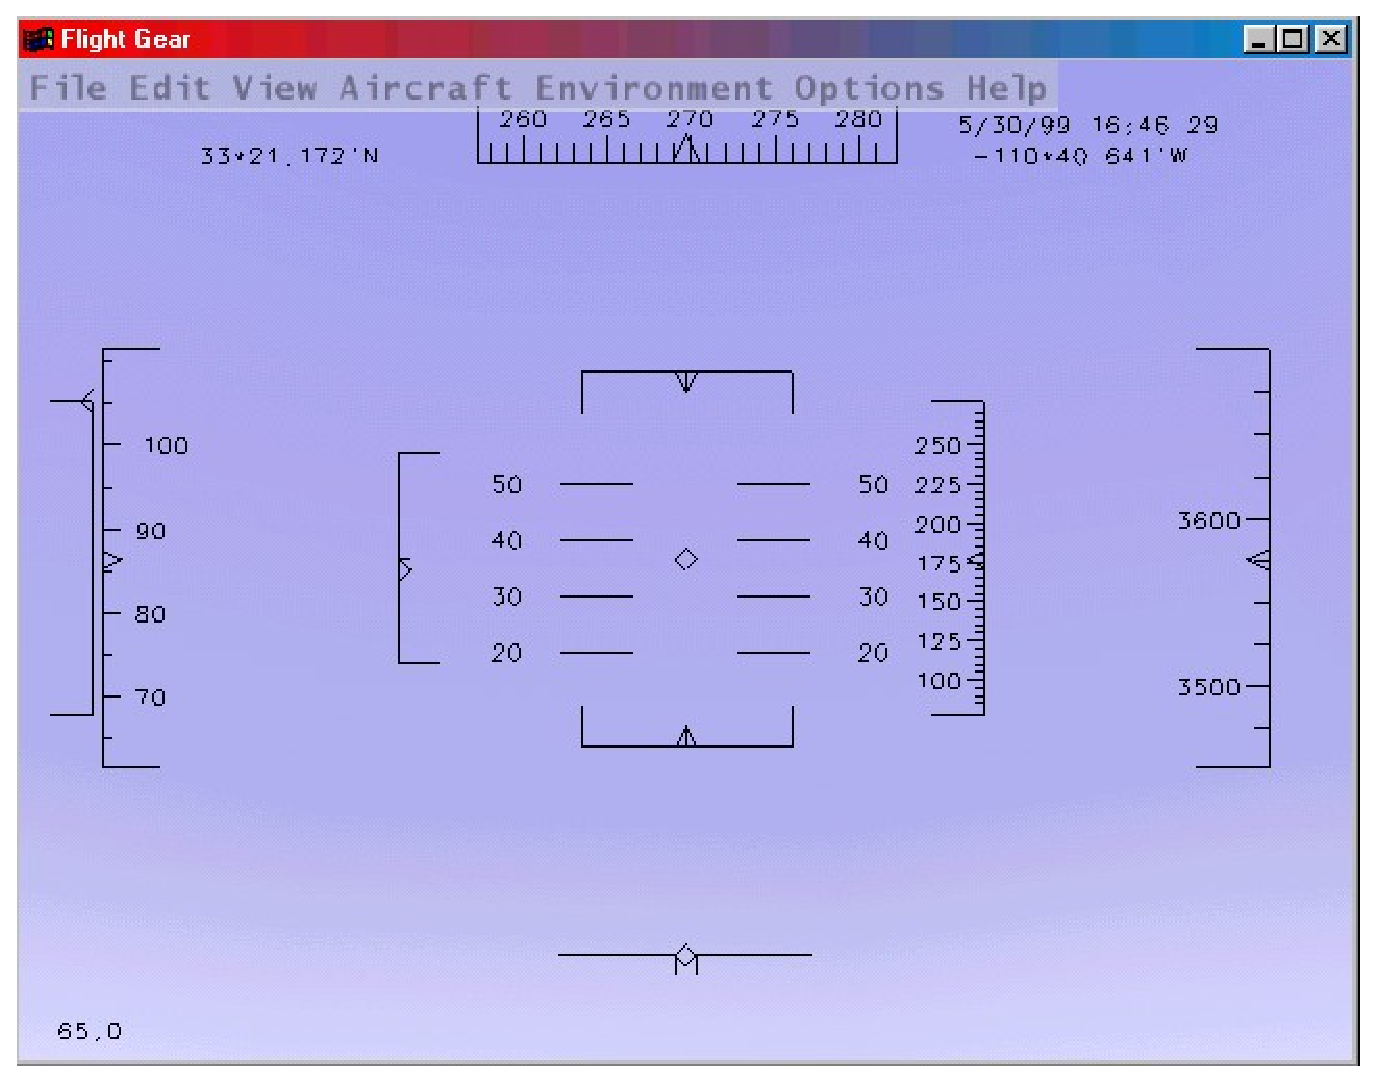
\includegraphics[clip,width=12.5cm]{hud.eps}
}

\smallskip
 \noindent
Fig.\,3: \textit{The HUD, or head up display.}
\medskip

The \Index{HUD} shown in Fig.\,3  displays all main flight parameters of the plane. In
the center you find the \Index{pitch indicator} (in degrees) with the \Index{aileron
indicator} above and the \Index{rudder indicator} below. A corresponding scale for the
elevation\index{elevation indicator} can be found to the left of the pitch scale. On the
bottom there is a simple \Index{turn indicator}.

There are two scales at the extreme left: The inner one displays the \Index{speed} (in
kts) while the outer one indicates position of the \Index{throttle}. You may recall the
\Index{Navion} taking off at a speed of 100 kts. The two scales on the extreme r.h.s
display your \Index{height}, i.\,e. the left one shows the height above ground while the
right of it gives that above zero, both being displayed in feet.

Besides this, the \Index{HUD} displays some additions information. On the upper right you
find date and time. Below, you see \Index{latitude} and \Index{longitude} of your current
position on the l.h.s and r.h.s, resp. In the lower left corner there is a number
indicating the \Index{frame rate}, i.e. the number of times the picture being re-drawn
each second.

You can change color of the \textbf{HUD} using the ''H'' key. Pressing it several times
minimizes the HUD.

\section{The Panel\index{panel}}

Besides the \Index{HUD}, \FlightGear has a \Index{panel} which can be activated by
pressing the ''P'' key. (It is recommended disabling the HUD then by pressing ''H''
several times.) While the panel is not yet fully complete the basic five \Index{flight
instruments} to scan are present and working.
\medskip

 \centerline{
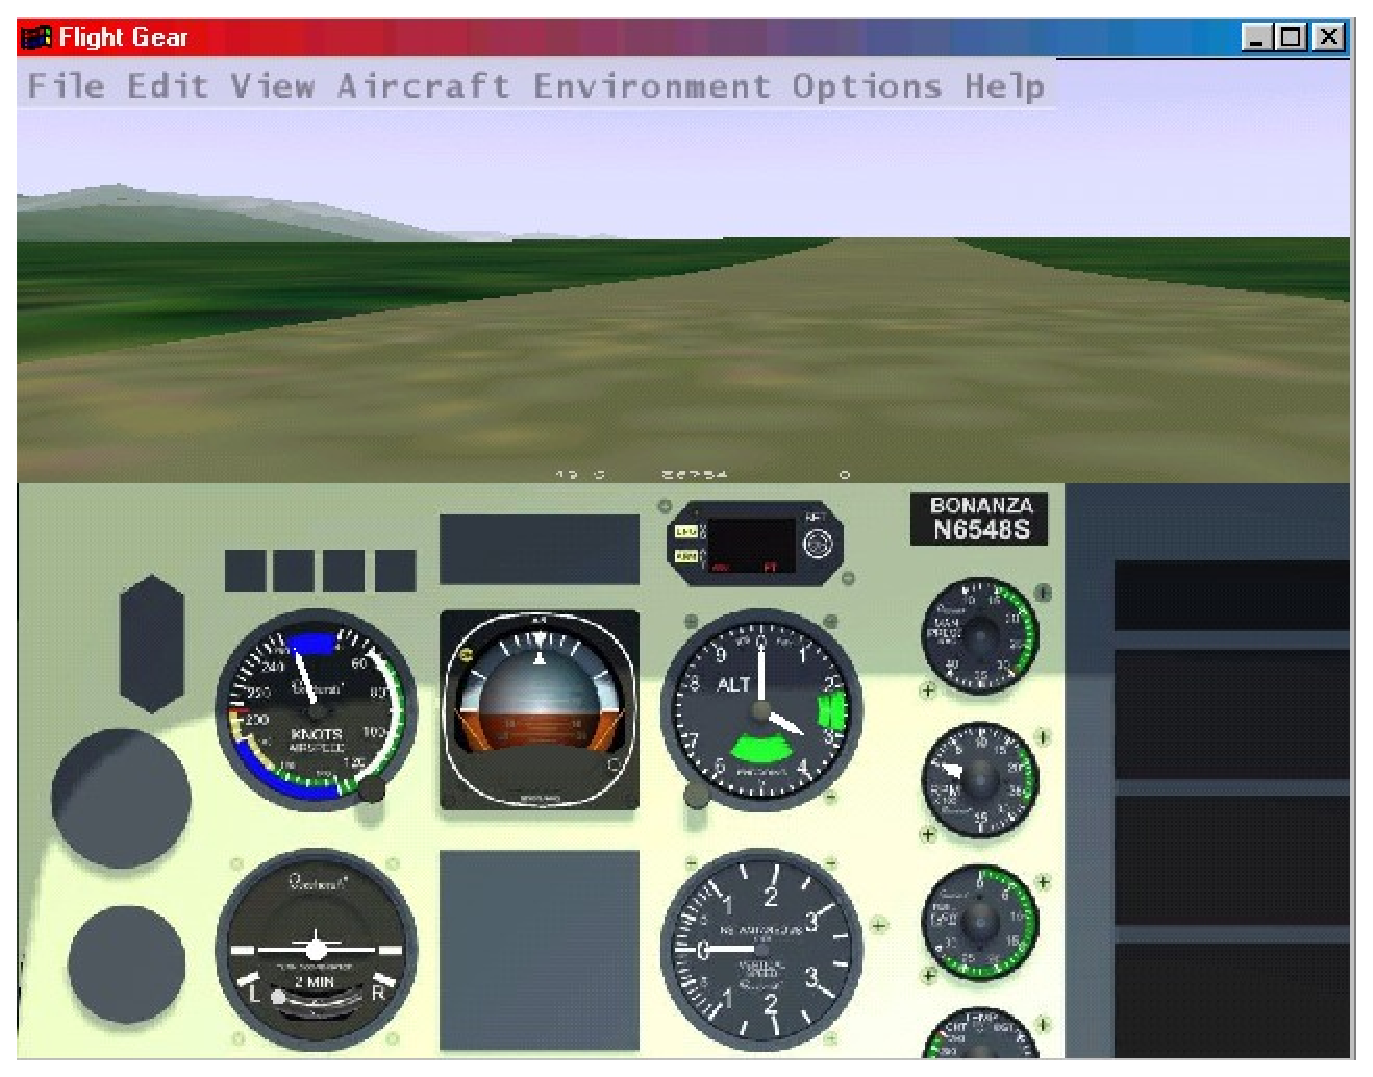
\includegraphics[clip,width=12.5cm]{panel.eps}
}

\smallskip
 \noindent
Fig.\,4: \textit{The panel.}
\medskip

In the center you find the \Index{artificial horizon} (attitude indicator) displaying
pitch and bank of your plane. It has pitch marks (hard to be seen in this version) as
well as bank marks at 10, 20, 30, 60, and 90 degrees.

Left to the artificial horizon, you'll see the \Index{airspeed indicator}. Not only does
it have a speed indication in knots (recall: The Navion takes off at 100 kts) but also
several arcs showing characteristic \Index{velocity rages} you have to consider. At
first, there is a green arc indicating the normal operating range of speed with the flaps
(net yet being implemented in \FlightGear) fully retracted. The white arc indicates the
range of speed with flaps in action. The tiny yellow arc shows a range, which should only
be used in smooth air. The upper end of it has a red radial indicating the speed never to
be exceeded.

Below the airspeed indicator you can find the \Index{turn indicator}. The airplane in the
middle indicates the roll of your plane. If the left or right wing of the plane is
aligned with one of the marks this indicates a standard turn, in which you make a full
360 degrees turn in exactly two minutes.

Below the plane, still in the turn indicator, is another instrument, called
\Index{inclinometer}. It indicates if \Index{rudder} and \Index{ailerons} are
coordinated. During turns, you always have to operate aileron and rudder in such a way
that the ball in the tube remains centered; otherwise the plane is skidding.

To the right of the artificial horizon you find the \Index{altimeter} showing the height
above sea level (not ground!). At present it is not yet working in
\FlightGear\hspace{-1mm}. Below the altimeter is the \Index{vertical speed indicator}
which, on the other hand, is operational. It indicates the rate of climbing or sinking of
your plane in hundreds of feet per minute.

There is one more instrument working in the panel, i.e. the second one in the column on
the r.h.s. indicating position of \Index{throttle}.

This completes description of the present main \FlightGear instruments. If you are
looking for some interesting places to discover with \FlightGear (which may or may not
require downloading additional scenery) you may want to check

 \web{http://www.flightgear.org/Downloads/Places}.

There is now a menu entry for entering directly the \Index{airport code} of the airport
you want to start from.

Finally, if you're done and are about to leave the plane, just hit the ESC key or use the
corresponding menu entry to exit the program.

%% Revision 0.00  1998/09/08  michael
%% Initial revision for version 0.53.
%% Revision 0.01  1998/09/20  michael
%% several extensions and corrections, added Fig.1.
%% revision 0.10  1998/10/01  michael
%% final proofreading for release
%% revision 0.11  1998/11/01  michael
%% Complete revision of keyborad controls, interesting places
%% revision 0.12  1999/03/07  michael
%% Corrected rudder key
%% revision 0.20  1999/06/04  michael
%% HUD completely rewritten, added panel section with picture, and menu section
%% updated keystrokes
